\section{Проектирование реализации}
Для разработки распределенной асинхронной системы обработки real-time финансовых данных было спроектировано две модели: c2 и c3.

На уровне C2 я разбил систему на контейнеры, каждый из которых содержит исполняемую и развертываемую подсистему. В этом случае, контейнеры представляют собой сервисы, отвечающие за определенную функциональность системы. Была разработана диаграмма контейнеров, на которой отображены все контейнеры, их взаимосвязи и зависимости друг от друга.

\begin{figure}[h]
    \centering
    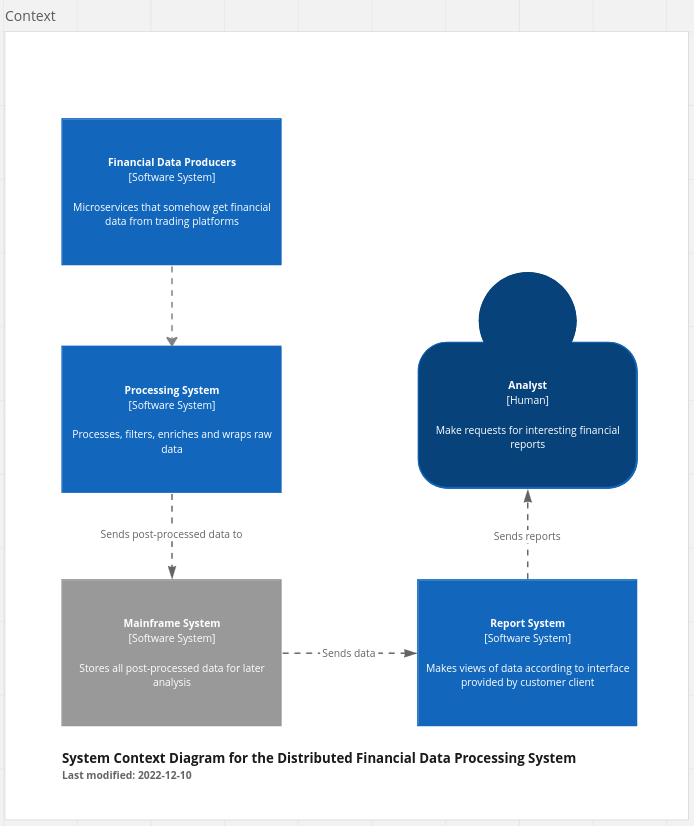
\includegraphics[width=0.8\columnwidth]{c2model.png}
    \caption{C2 модель архитектуры}
\end{figure}


На уровне C3 я разделил контейнеры на компоненты и отразил связи между компонентами и другими контейнерами или системами. В данной модели я сосредоточился на взаимодействии сервисов с помощью Apache Kafka. Каждый сервис отправляет сообщения на Kafka, которые затем обрабатываются другими сервисами. Была разработана диаграмма компонентов, на которой отображены все компоненты системы, их взаимосвязи и связи с другими системами.


\begin{figure}[h]
    \centering
    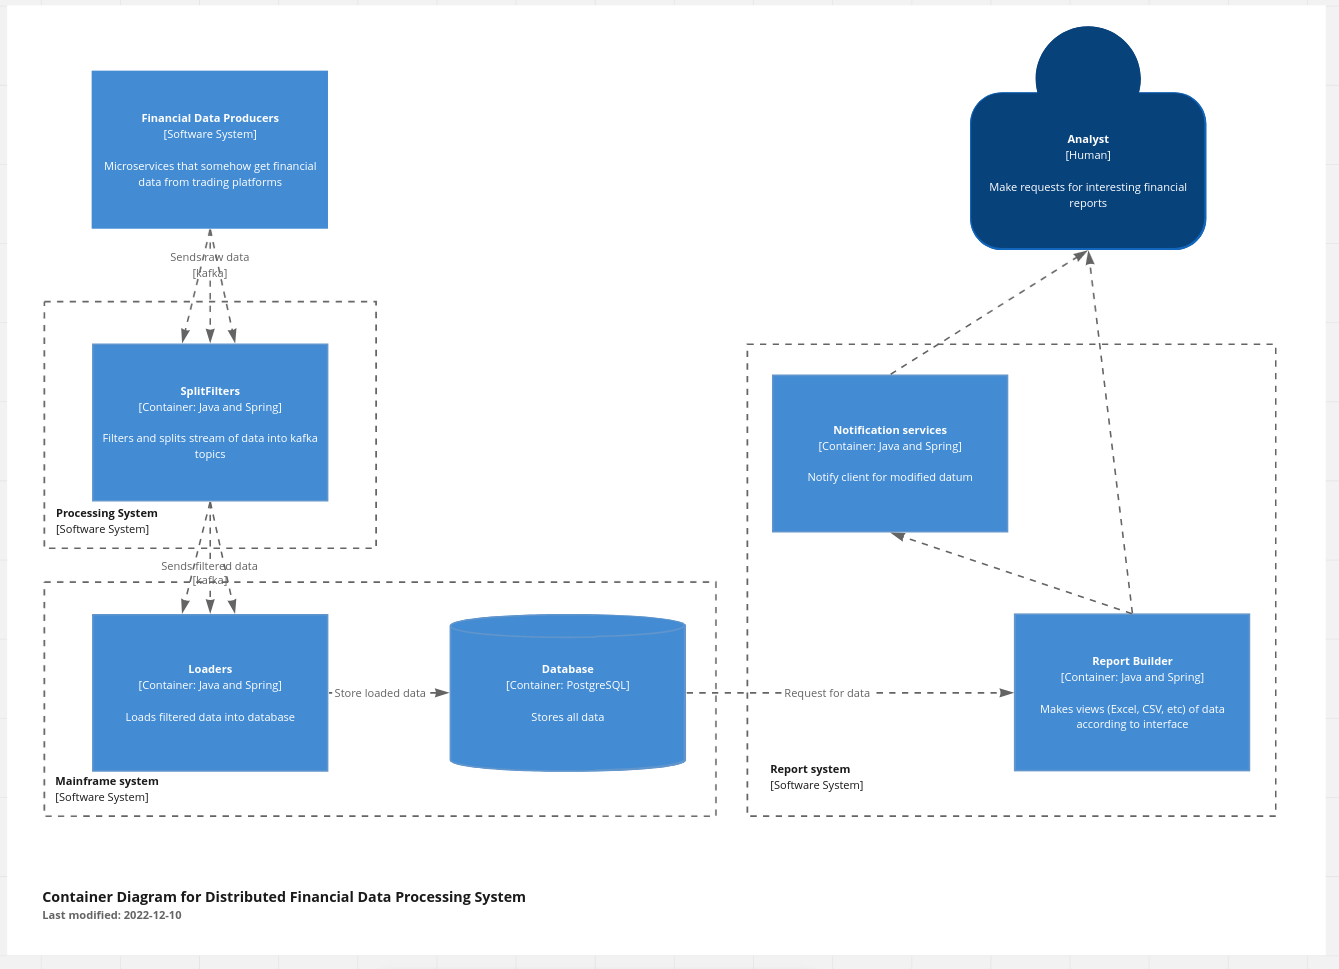
\includegraphics[width=0.8\columnwidth]{c3model.png}
    \caption{C3 модель архитектуры}
\end{figure}

Обе модели позволяют наглядно представить архитектуру системы и понять, как каждый компонент взаимодействует с другими компонентами и системами.